\section{Data Preprocessing}

\subsection{Downsampling the Data}
As the purpose of using Dirichlet Multinomial Regression was to be able to model the distribution of habitat label occurrences over an area, we downsampled the combined 2011, 2015 dataset which was at a significantly higher resolution than the 2009 dataset \todo{(calculate how much perhaps)}. To do this, a `grid' of squares was essentially mapped onto original space, and points in each grid grouped together into a single point. For the multi-output labels, all label counts in each lower-resolution grid were summed, whereas for the single label case, the label was selected randomly \textit{but} with more weighting to the non-sand labels, to slightly increase the variance of labels observed. The reason for doing this was because of the dominance of the 'sand` habitat - random selection when only one absolute label per point was present resulted in an even larger portion of sand than in the original dataset, causing predictions on the full query data to sometimes result in almost $100\%$ sand, even moreso than was already the case in \Cref{fig:det4maps}.

% Two methods of downsampling in particular were tested. The first coarser approach involved simply taking the space in which the data was collected and placing grids of fixed size over them as in \cref{fig:gridsplit}, binning all points falling within each grid into a single datapoint. Each of these data points contained multiple points from the original dataset with their own counts for each of the possible labels, so the downsampled points simply took the sum of all the label counts in each fixed grid. 
% 
% The second summed label counts in the same way, but clusters were instead formed by first calculating the full dendrogram on the 16502 entries in the training data, and forming groups such that none had more than 5 of the original points within them, and the sub-clusters (at each level of the dendrogram) were no more than a 21 metres away from one another. As can be seen in \cref{fig:dendrogram}, the gradual merging into the single supercluster was quite consistent, indicating the original datapoints were mostly evenly distributed.
% 
% \todo{(cut down this section (probably down to one paragraph) - and also talk about how for the single label case, instead of summing counts for the new 'label', labels were chosen at random (for more variance in the GP which is otherwise too certain about everything being sand))}
% 
\begin{figure}[H]
    \includegraphics[scale=0.55]{training_map_fixedgrid.pdf}
    \caption{Fixed-sized grids placed over training data \todo{(redo this plot nicely!)}}
    \label{fig:gridsplit}
\end{figure} 

% \begin{figure}[H]
%     \centering
%     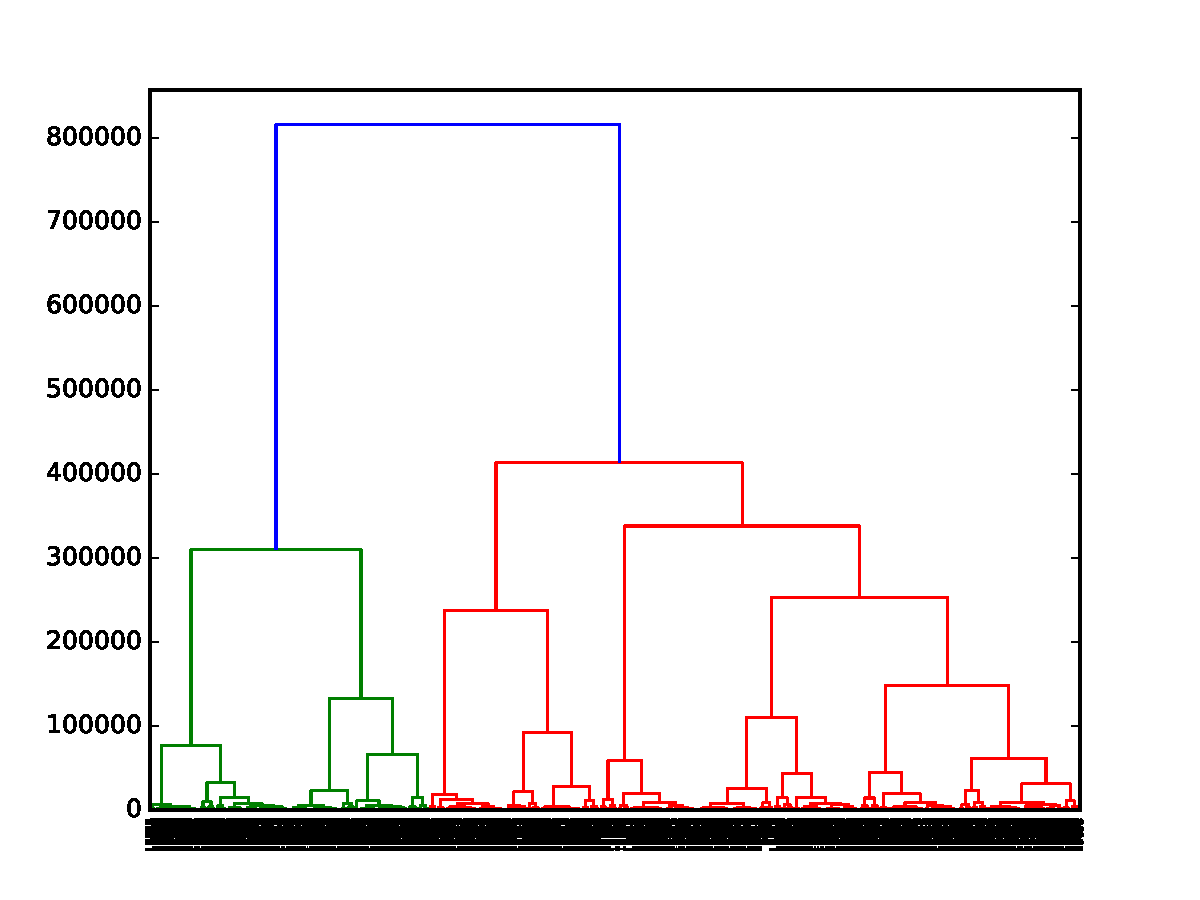
\includegraphics[scale=0.6]{dendrogram.pdf}
%     \caption{Dendrogram of training data}
%     \label{fig:dendrogram}
% \end{figure}

\subsection{Simplifying labels}
Another preprocessing step that was performed was the aggregation of habitat labels. The original training data contained 24 separate labels determined through an automated clustering procedure using Dirichlet Processes. Because of the uneven distribution of these labels (\Cref{fig:singlelabeldistr} and \Cref{fig:multilabeldistr}), with the occurrence of some too insignificant for any machine learning algorithms to pick up, they were simplified in collaboration with ecological experts, who manually identified which of the 24 labels were in fact of the same class - for example, 5 separate classes of coral may have been indistinguishable to the average person, and were hence grouped into a single label. This allowed the near-non-occurring labels to be grouped together with more commonly occurring ones, whilst also allowing a different level of granularity in training models/forming predictions that could be used if only an approximation equivalent to observable human differences of an area's benthic map were required. Moreover, due to the unsupervised nature of the labeling, certain clusters were notably \textit{inconsistent} with the rest, for example when sea cucumbers became the identifying feature of one of the 24 labels.

\begin{table}[H]
    \centering
    \begin{tabular}{|c| c|}
        \hline
        simplified & original \\\hline
        0 & 1, 2, 18, 20, 21, 23, 24 \\
        1 & 3, 5, 10, 16, 17, 19, 22\\
        2 & 13, 14, 15 \\
        3 - Sand & 4, 6, 7, 8, 9, 11, 12 \\
        \hline
    \end{tabular}
    \caption{Full-simplified label mappings \tiny{\todo{label mappings - sand, coral, patchy coral, (?) halameda, rhodliths}}}
    \label{table:labelmappings}
\end{table}

\begin{figure}
    \includegraphics[scale=0.17]{class_mosaic_24_classes.jpg}
    \caption{Samples of images from each of the full 24 classes \todo{mark with the simplified labels adjacent to it}}
    \label{fig:24classes}
\end{figure}

\begin{figure}
    \includegraphics[scale=0.17]{class_mosaic_5_classes.png}
    \caption{Samples of images from each of summarised 4 classes \todo{mark with the simplified labels adjacent to it}}
    \label{fig:4classes}
\end{figure}

\begin{figure}[H]
    \begin{minipage}{.47\linewidth}
        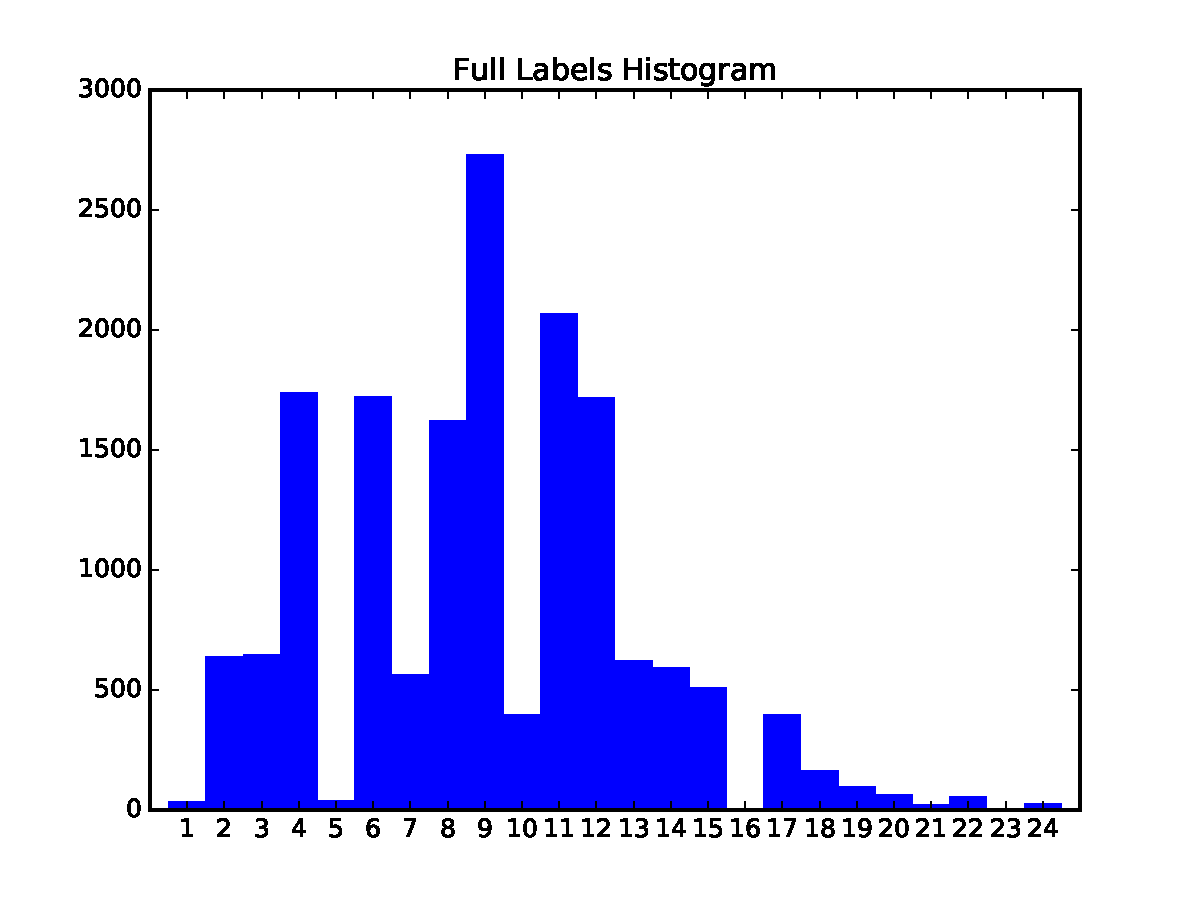
\includegraphics[width=\linewidth]{hist_full_labels.pdf}
        \caption{Distribution of labels in original dataset}
        \label{fig:singlelabeldistr}
    \end{minipage}
    \hfill
    \begin{minipage}{.47\linewidth}
        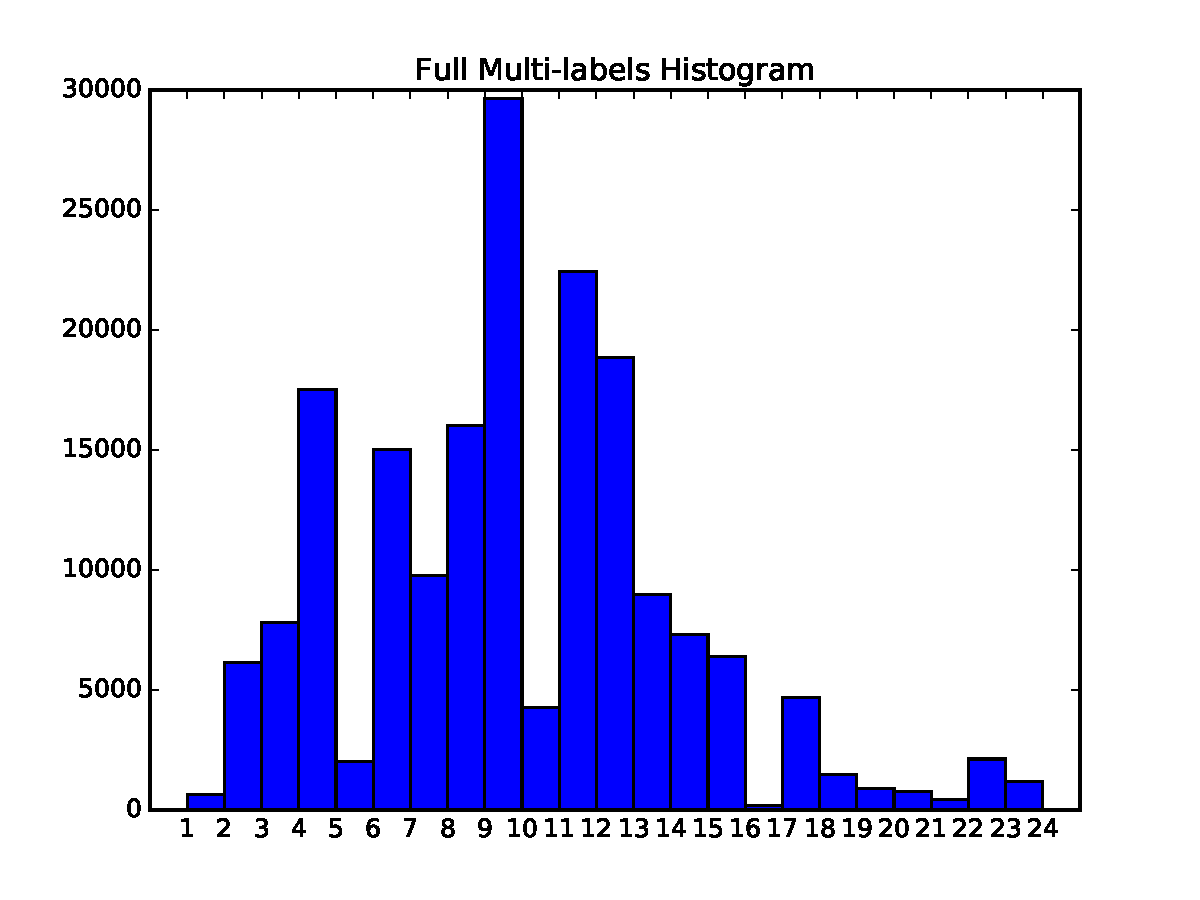
\includegraphics[width=\linewidth]{hist_full_multi_labels.pdf}
        \caption{Distribution of labels in multi-label outputs}
        \label{fig:multilabeldistr}
    \end{minipage}
\end{figure}

\begin{figure}[H]
    \begin{minipage}{.47\linewidth}
        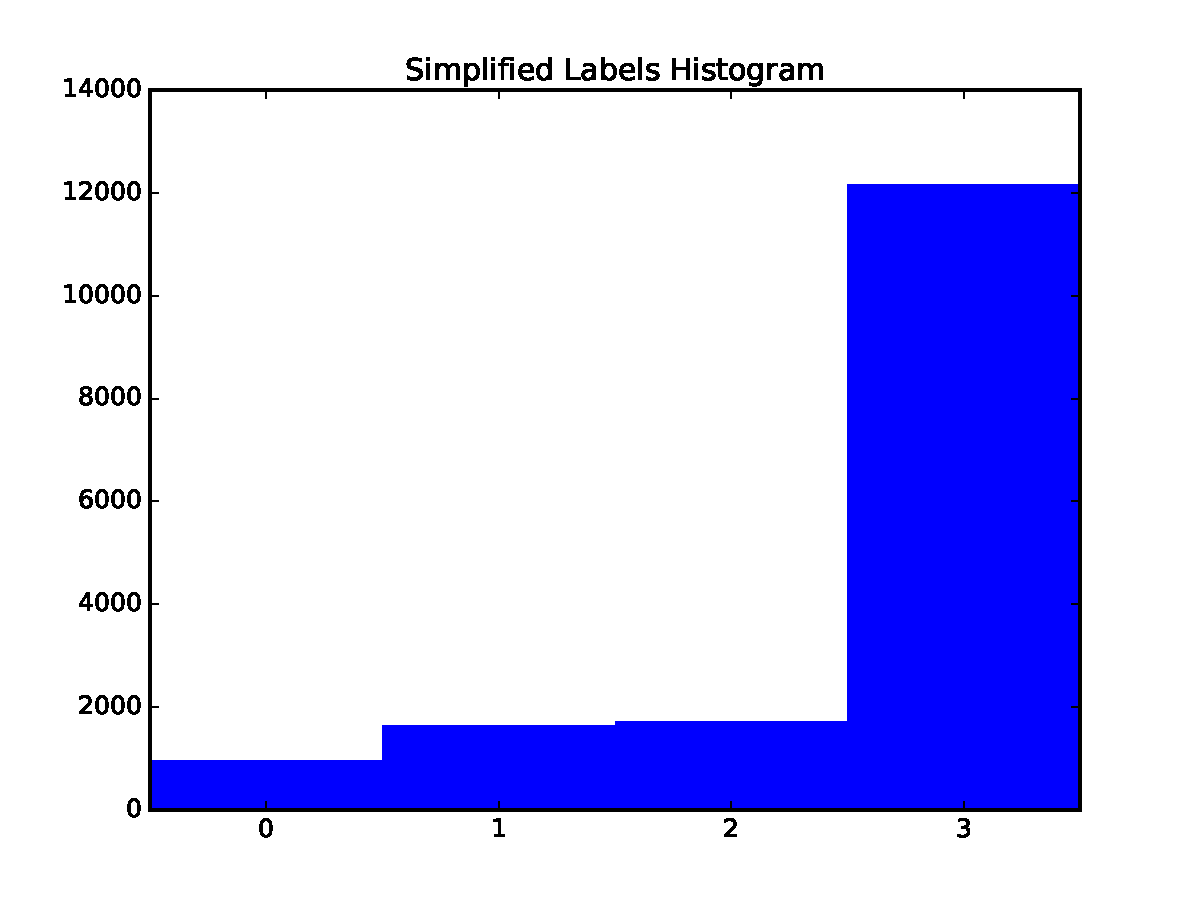
\includegraphics[width=\linewidth]{hist_simple_labels.pdf}
        \caption{Distribution of simplified labels in original dataset}
        \label{fig:singlelabeldistr}
    \end{minipage}
    \hfill
    \begin{minipage}{.47\linewidth}
        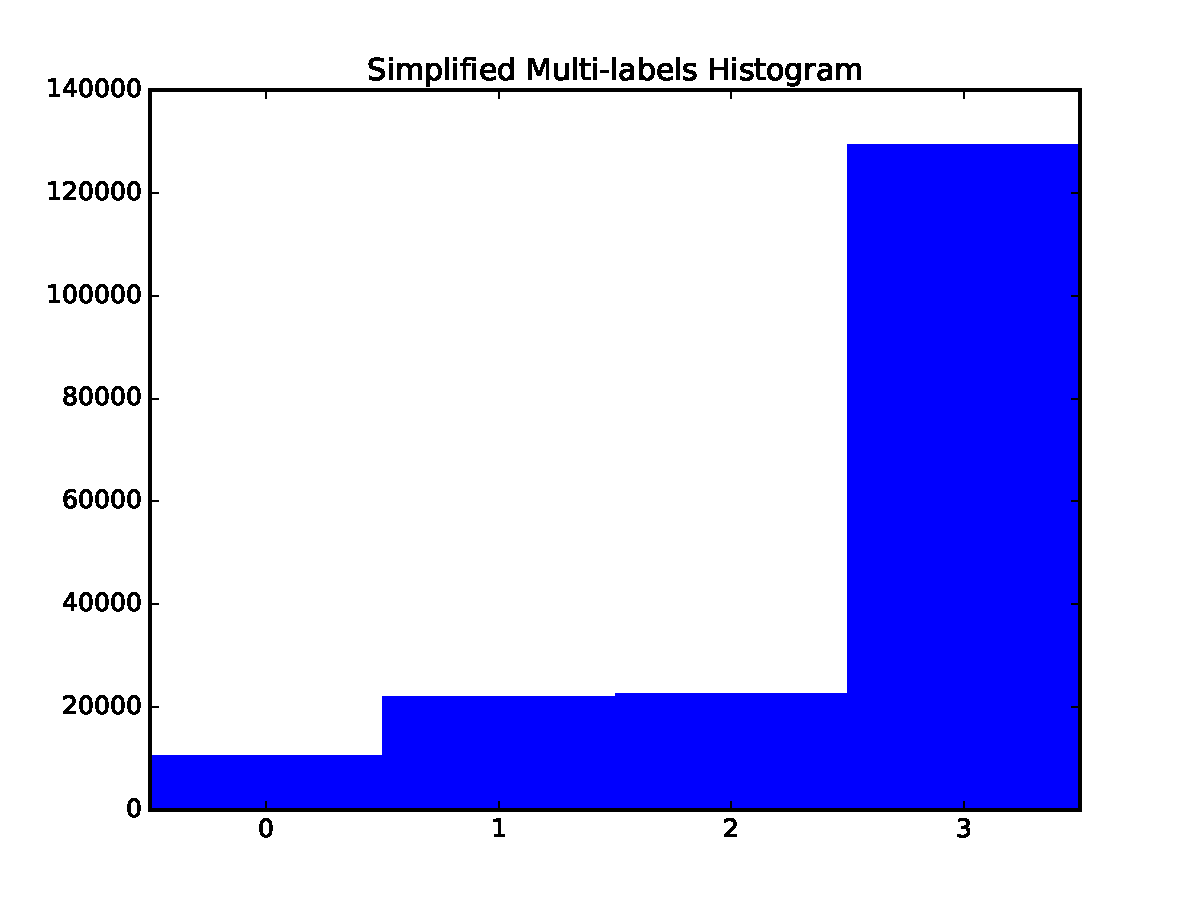
\includegraphics[width=\linewidth]{hist_simple_multi_labels.pdf}
        \caption{Distribution of simplified labels in multi-label outputs}
        \label{fig:multilabeldistr}
    \end{minipage}
\end{figure}

Note that from this point onwards, we will be working with the reduced feature set, in line with the aim of the paper to show the advantages of dirichlet multinomial regression when studies (environmental or otherwise) are limited to lower resolution data where strictly assigning only a single label to the features at a given data point is not representative of the otherwise rich information available. This restriction is a realistic one, because to be able to monitor large portions of the ocean for conservational and management reasons amongst others, data needs to be collected economically en-masse - and this means not collecting very high resolution data that would attract large costs at scale.

% \subsection{Coordinates as features}
% Due to the abundant bathymetry data that was available in the form of depth, rugosity and aspect at each available data point, the coordinates themselves were not included in the feature space for experiments. Whilst it is logical that in a natural environment, areas that were spatially close would also have similar properties, this should not be relied upon, and other intrinsic properties should be the basis upon which predictions are made. Forming predictions on the full query dataset using a random forest supports this notion quite strongly - whilst 10-fold cross validation using the coordinates as features had a notably higher F-score of 0.61 compared to 0.40 without, the unnaturally straight split between the left and right segments (\Cref{fig:rf_w_coords_preds}) over a 12km region suggests that the predictive map is flawed. Moreover, by including the coordinates as a training feature, an assertion is made about the direct relationship between a benthic location and the habitat class/es it contains, despite its other physical properties such as depth, aspect, etc - an assumption that should not be embedded into the model before fitting it to the data even begins.
% 
% \begin{figure}[H]
%     \begin{minipage}{.49\linewidth}
%         \includegraphics[width=\linewidth]{full_predictions_randomforest.pdf}
%         \caption{Full predictive map using Random Forests including coordinates as features}
%         \label{fig:rf_w_coords_preds}
%     \end{minipage}
%     \hfill
%     \begin{minipage}{.49\linewidth}
%         \includegraphics[width=\linewidth]{full_predictions_randomforest_nocoords.pdf}
%         \caption{Full predictive map using Random Forests excluding coordinates as features}
%         \label{fig:rf_wo_coords_preds}
%     \end{minipage}
% \end{figure}

\subsection{Preprocessing and Feature Projection}
To maximise performance of the algorithms used across the experiments, a number of preprocessing steps were taken to improve the predictions made. The features in the data were first scaled, where each feature was centred to the mean with unit variance), then normalised over each future such that they had unit length \todo{(include plots of the diff approaches across DM/GP/others, ref plots)}. To allow the algorithms tested to learn the data and its complexities better, projecting the data into higher dimensional space was required. Full quadratic projections ($x_0, x_1, x_2 \Rightarrow x_0^2 ,x_1^2 ,x_2 ,2x_0x_1 ,2x_0x_2 ,2x_1x_2$) and squared terms with a $1$ bias terms ($x_0, x_1, x_2 \Rightarrow x_0 + x_1 , x_2 ,x_0^2 ,x_1^2, x_2^2, 1$) were both tested. The latter was chosen, one of the reasons being that it resulted in an lower average error when performing 10-fold cross-validation using Dirichlet Multinomial Regression (\Cref{table:dmbasicresults}). It was also chosen to allow predictions to run faster, and for the Markov Chain Monte Carlo for Dirichlet Multinomial Regression later in this chapter, \textbf{significantly} reduce the number of dimensions that need to be traversed - considering the number of weights required is features $\times$ number of labels, this would correspond to the 4-label data needing $19*4=76$ vs $55*4=220$ weights, and the full 24-label case requiring $19*24=456$ vs $55*24=1320$ weights.

\todo{(ref plots)}

\todo{(show plots)}

% The results from the Experiments detailed in Chapter 4 are listed below. The range of possible class values in some cases have been stretched beyond the existing class labels so that values align between different outputs to allow for easy, direct visual comparison \todo{(this hasn't actually happened yet)}. Note that the results to the above experiments will include those of both non-downsampled and downsampled results, as well as the full set of 24 labels as well as simplified ones.
% 
% Due to the low occurrence of some labels in the original dataset though, they have ended up being ommitted in predictions - these are excluded from the colour schemes of the benthic maps generated, so that those that do occur can be given more distinct colours from one another as to better differentiate between the habitats of a map, as well as allow a consistent comparison of across different maps. \todo{(again, hasn't happened yet)}

% The associated generated maps from the experiments are also provided here, but proper evaluation of them, such as what habitat clusters and relationships can be gleaned, will be explored in Chapter 5. 

